\documentclass[12pt]{article}

\usepackage{amssymb,amsmath,amsfonts,booktabs,eurosym,float,geometry,ulem,graphicx,caption,color,setspace,sectsty,comment,footmisc,caption,multicol, multirow,natbib,pdflscape,subfigure,array,hyperref, pdflscape}

\normalem

\onehalfspacing
\newtheorem{theorem}{Theorem}
\newtheorem{corollary}[theorem]{Corollary}
\newtheorem{proposition}{Proposition}
\newenvironment{proof}[1][Proof]{\noindent\textbf{#1.} }{\ \rule{0.5em}{0.5em}}

\newtheorem{hyp}{Hypothesis}
\newtheorem{subhyp}{Hypothesis}[hyp]
\renewcommand{\thesubhyp}{\thehyp\alph{subhyp}}

\newcommand{\red}[1]{{\color{red} #1}}
\newcommand{\blue}[1]{{\color{blue} #1}}

\newcolumntype{L}[1]{>{\raggedright\let\newline\\arraybackslash\hspace{0pt}}m{#1}}
\newcolumntype{C}[1]{>{\centering\let\newline\\arraybackslash\hspace{0pt}}m{#1}}
\newcolumntype{R}[1]{>{\raggedleft\let\newline\\arraybackslash\hspace{0pt}}m{#1}}

\geometry{left=1.0in,right=1.0in,top=1.0in,bottom=1.0in}

\begin{document}

\begin{titlepage}
\title{Arjun Shanmugam's Senior Thesis}
\author{Arjun Shanmugam}
\date{\today}
\maketitle
\begin{abstract}
\noindent Placeholder\\


\bigskip
\end{abstract}
\setcounter{page}{0}
\thispagestyle{empty}
\end{titlepage}
\pagebreak \newpage




\doublespacing


\section{Introduction} \label{sec:introduction}

\section{Literature Review} \label{sec:literature}

\section{Data} \label{sec:data}
    \subsection{Evictions Data}
        \begin{figure}
            \centering
            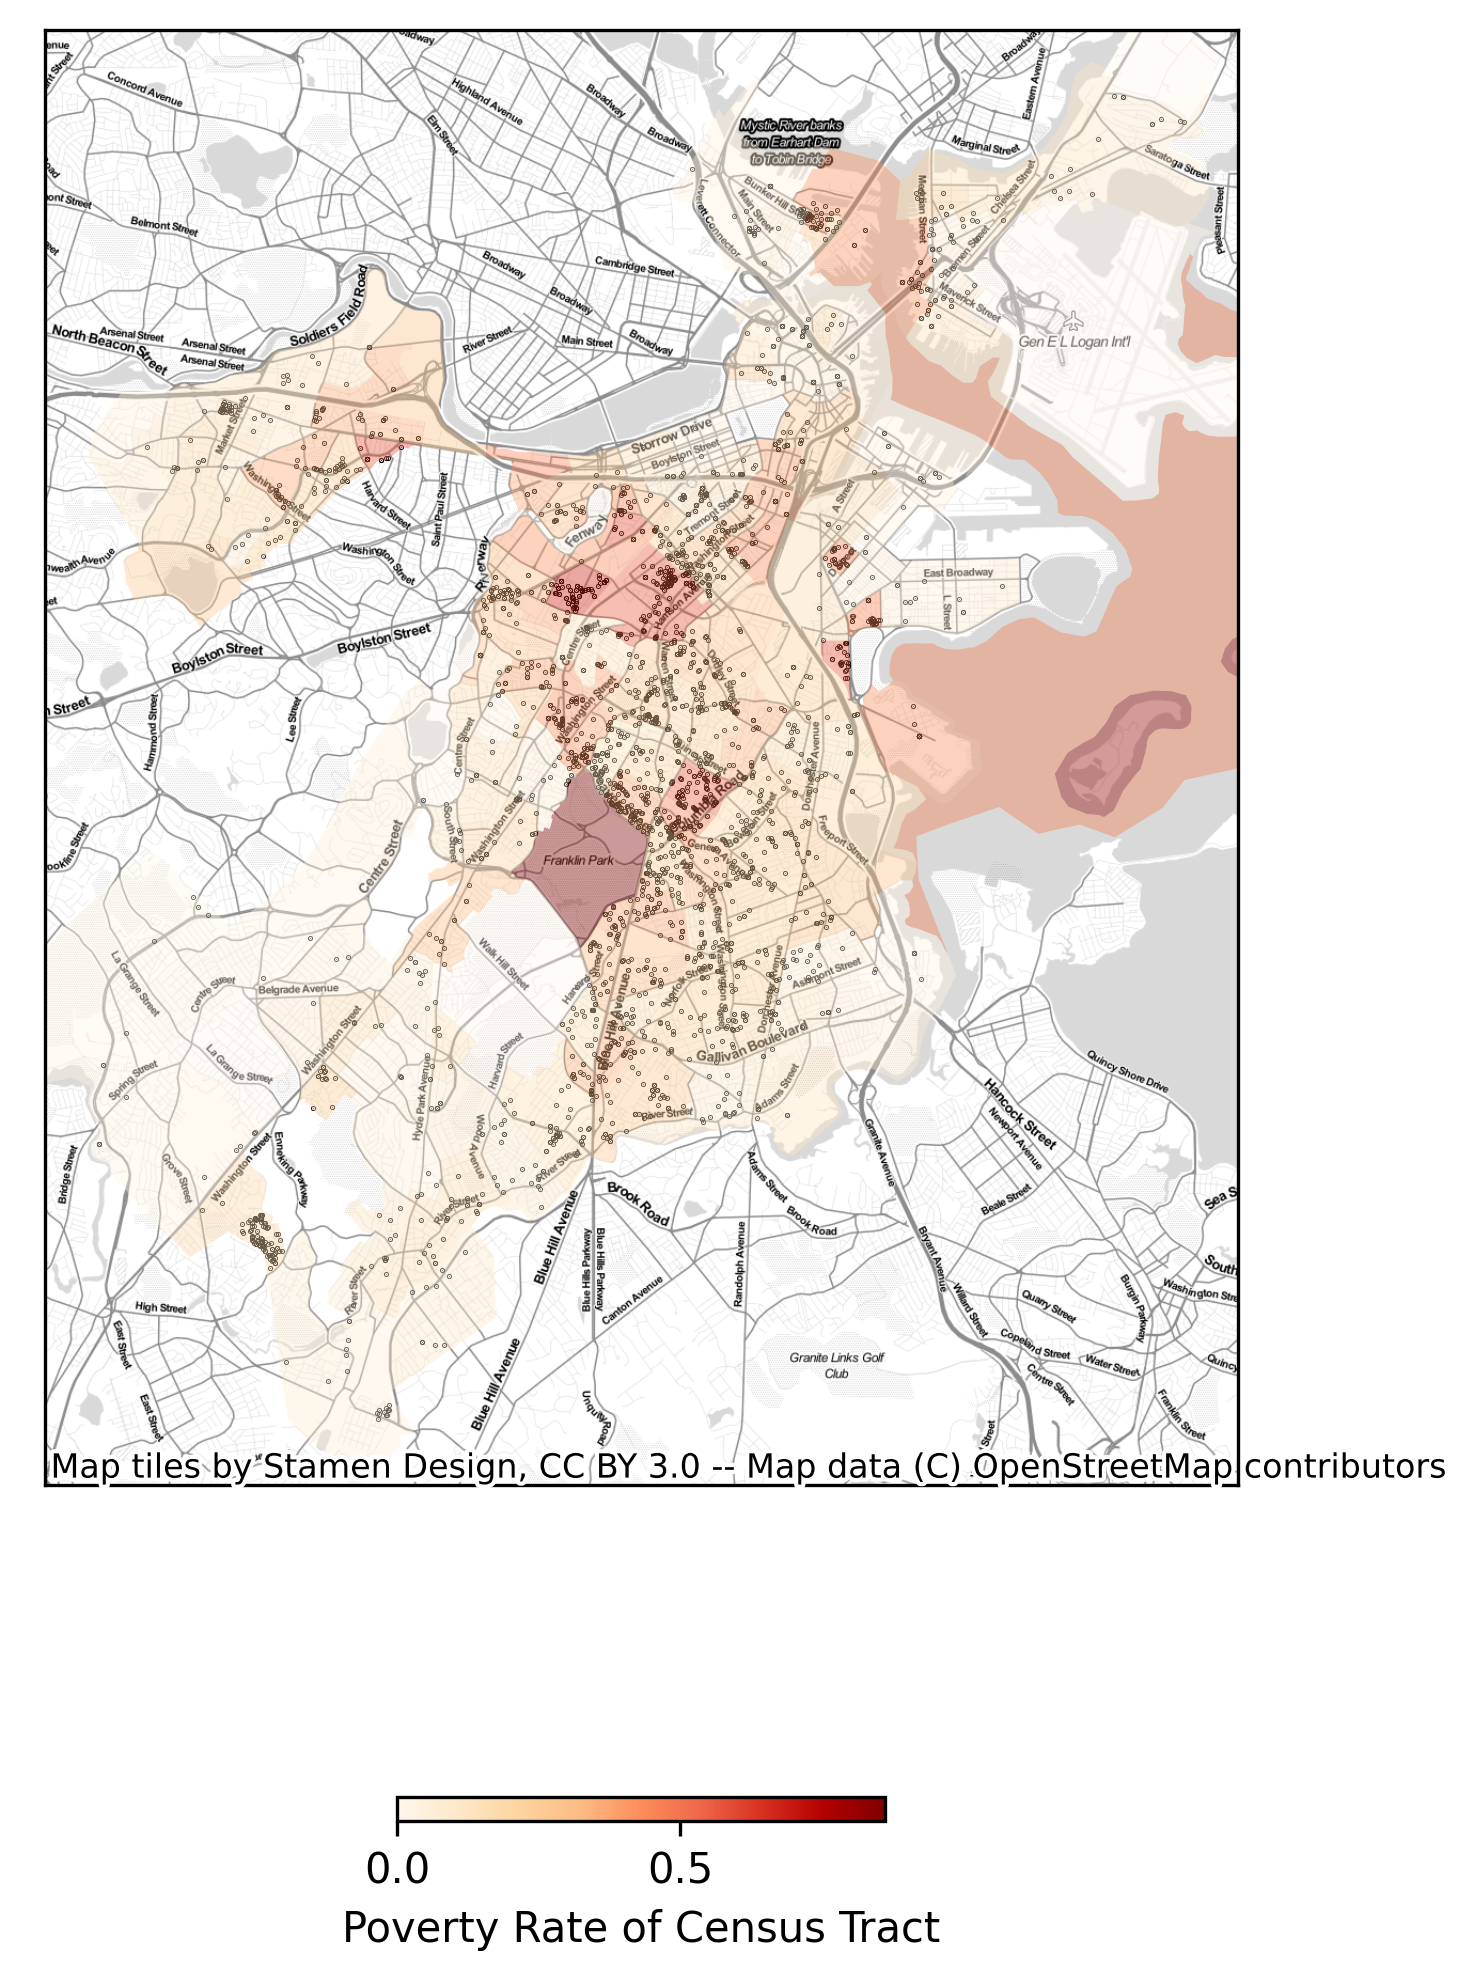
\includegraphics{output/summary_statistics/figures/evictions_map.png}
            \caption{Caption}
            \label{fig:my_label}
        \end{figure}
    \subsection{Tax Assessment Records}
    \subsection{Zestimates}
    
    \begin{landscape}
    \subsection{Summary Statistics}
         \begin{table}[H]
            \centering
            \small
            \begin{tabular}{llcccc}
\toprule
 &  & Mean & Median & S.D. & N \\
Panel & Variable &  &  &  &  \\
\midrule
\multirow[c]{3}{4cm}{\textit{Panel A: Case Initiation}} & For cause & 0.12 & 0.00 & 0.33 & 40,727 \\
 & No cause & 0.11 & 0.00 & 0.31 & 40,727 \\
 & Non-payment of rent & 0.75 & 1.00 & 0.43 & 40,727 \\
\cline{1-6}
\multirow[c]{6}{4cm}{\textit{Panel B: Case Resolution}} & Case defaulted & 0.20 & 0.00 & 0.40 & 40,727 \\
 & Case dismised & 0.29 & 0.00 & 0.45 & 40,727 \\
 & Case duration & 57.81 & 21.00 & 78.29 & 39,087 \\
 & Case heard & 0.06 & 0.00 & 0.23 & 40,727 \\
 & Case mediated & 0.41 & 0.00 & 0.49 & 40,727 \\
 & Money judgment & 1,890.34 & 0.00 & 5,279.49 & 40,727 \\
\cline{1-6}
\multirow[c]{4}{4cm}{\textit{Panel C: Defendant and Plaintiff Characteristics}} & Defendant has an attorney & 0.09 & 0.00 & 0.28 & 40,727 \\
 & Defendant is an entity & 0.01 & 0.00 & 0.08 & 40,727 \\
 & Plaintiff has an attorney & 0.84 & 1.00 & 0.37 & 40,727 \\
 & Plaintiff is an entity & 0.70 & 1.00 & 0.46 & 40,727 \\
\cline{1-6}
\multirow[c]{4}{4cm}{\textit{Panel D: Assessor Records From Most Recent Pre-Filing F.Y.}} & Building value & 8,350,204.19 & 636,500.00 & 22,073,916.94 & 36,587 \\
 & Land value & 2,471,065.61 & 192,400.00 & 6,218,383.08 & 36,587 \\
 & Other value & 112,575.80 & 1,000.00 & 659,661.29 & 36,587 \\
 & Total property value & 10,900,678.30 & 954,900.00 & 26,482,630.60 & 36,587 \\
\cline{1-6}
\multirow[c]{4}{4cm}{\textit{Panel E: Census Tract Characteristics}} & Median household income (2016) & 52,659.44 & 47,105.00 & 27,177.48 & 40,726 \\
 & Median two bedroom rent (2015) & 1,116.27 & 1,055.00 & 396.29 & 30,537 \\
 & Population density (2010) & 9,159.77 & 5,978.61 & 9,574.14 & 40,726 \\
 & Portion white (2010) & 0.58 & 0.63 & 0.29 & 40,726 \\
\cline{1-6}
\multirow[c]{9}{4cm}{\textit{Panel F: Zestimates Around Filing Date}} & Filing date & 377,384.02 & 305,144.00 & 316,645.29 & 10,096 \\
 & Five years before filing date & 261,462.86 & 213,270.60 & 238,040.64 & 9,842 \\
 & Four years before filing date & 280,243.32 & 225,065.75 & 276,051.45 & 9,968 \\
 & One year after filing date & 421,601.75 & 347,550.00 & 344,328.86 & 10,443 \\
 & One year before filing date & 351,172.05 & 278,722.25 & 311,982.74 & 10,190 \\
 & Three years after filing date & 501,611.80 & 414,600.00 & 780,467.01 & 5,894 \\
 & Three years before filing date & 307,137.16 & 240,097.38 & 369,763.53 & 10,172 \\
 & Two years after filing date & 477,948.08 & 393,900.00 & 457,694.83 & 9,175 \\
 & Two years before filing date & 341,084.08 & 259,176.00 & 987,145.51 & 10,182 \\
\cline{1-6}
\bottomrule
\end{tabular}

            \caption{Summary Statistics}
            \label{tab:table_1}
        \end{table}

        \newpage
        \begin{table}[H]
            \centering
            \small
            \begin{table}[H]
\begin{tabular}{llrrrr}
\toprule
 &  & \multicolumn{2}{c}{Control Group} & \multicolumn{2}{c}{Treatment Group} \\
 &  & Mean & N & Mean & N \\
Panel & Variable &  &  &  &  \\
\midrule
\multirow[c]{8}{4cm}{\textit{Panel A: Case Initiation}} & For cause & 0.12 & 3651 & 0.12 & 10708 \\
 & For cause (transfer) & 0.01 & 3651 & 0.01 & 10708 \\
 & Foreclosure & 0.01 & 3651 & 0.03 & 10708 \\
 & Foreclosure (transfer) & 0.00 & 3651 & 0.00 & 10708 \\
 & No cause & 0.12 & 3651 & 0.10 & 10708 \\
 & No cause (transfer) & 0.02 & 3651 & 0.00 & 10708 \\
 & Non-payment of rent & 0.69 & 3651 & 0.72 & 10708 \\
 & Non-payment of rent (transfer) & 0.03 & 3651 & 0.01 & 10708 \\
\cline{1-6}
\multirow[c]{5}{4cm}{\textit{Panel B: Case Resolution}} & Case defaulted & 0.00 & 3651 & 0.70 & 10708 \\
 & Case involuntarily dismissed & 0.99 & 3651 & 0.00 & 10708 \\
 & Case heard & 0.01 & 3651 & 0.21 & 10708 \\
 & Case mediated & 0.00 & 3651 & 0.00 & 10708 \\
 & Case voluntarily dismissed & 0.00 & 3651 & 0.00 & 10708 \\
\cline{1-6}
\multirow[c]{5}{4cm}{\textit{Panel C: Defendant and Plaintiff Characteristics}} & Defendant has an attorney & 0.22 & 3651 & 0.07 & 10708 \\
 & Plaintiff has an attorney & 0.78 & 3651 & 0.81 & 10708 \\
 & Defendant is an entity & 0.01 & 3651 & 0.01 & 10708 \\
 & Plaintiff is an entity & 0.62 & 3651 & 0.67 & 10708 \\
 & Money judgment & 63.61 & 3651 & 3688.76 & 10708 \\
\cline{1-6}
\multirow[c]{5}{4cm}{\textit{Panel C: Assessor Records From Post-Filing F.Y.}} & Total property value & 6478531.48 & 1256 & 8995455.63 & 3992 \\
 & Building value & 1605427.57 & 1256 & 2352344.15 & 3992 \\
 & Land value & 61247.49 & 1256 & 100993.11 & 3992 \\
 & Other value & 8138231.73 & 1256 & 11437647.57 & 3992 \\
 & Units & 41.23 & 1256 & 42.09 & 3992 \\
\cline{1-6}
\multirow[c]{9}{4cm}{\textit{Panel E: Zestimates Around Treatment}} & Five years before latest docket date & 252041.76 & 865 & 279947.69 & 2362 \\
 & Four years before latest docket date & 279493.58 & 875 & 302370.92 & 2388 \\
 & Three years before latest docket date & 308864.59 & 885 & 324126.19 & 2423 \\
 & Two years before latest docket date & 331594.86 & 888 & 348565.94 & 2427 \\
 & One year before latest docket date & 343934.24 & 906 & 372571.00 & 2447 \\
 & Latest docket date & 387984.48 & 920 & 422781.76 & 2471 \\
 & One year after latest docket date & 428426.83 & 899 & 467437.35 & 2402 \\
 & Two years after latest docket date & 451677.43 & 483 & 507407.77 & 1656 \\
 & Three years after latest docket date & 514122.00 & 250 & 502458.89 & 924 \\
\cline{1-6}
\bottomrule
\end{tabular}
\end{table}

            \caption{Balance Table}
            \label{tab:my_label}
        \end{table}
    \end{landscape}
       
\section{Results} \label{sec:result}

\section{Discussions} \label{sec:discussion}

\section{Conclusion} \label{sec:conclusion}



\singlespacing
\setlength\bibsep{0pt}
\bibliographystyle{my-style}
\bibliography{Placeholder}



\clearpage

\onehalfspacing

\section*{Tables} \label{sec:tab}
\addcontentsline{toc}{section}{Tables}



\clearpage

\section*{Figures} \label{sec:fig}
\addcontentsline{toc}{section}{Figures}




\clearpage

\section*{Appendix A. Placeholder} \label{sec:appendixa}
\addcontentsline{toc}{section}{Appendix A}



\end{document}